\chapter{Tight hardness bounds for the \mwccs{} problem}
\label{chap:hard}

	In this chapter, we will outline the frontier of complexity that characterizes the \textsc{Maximum-Weight Cross-Connected Subgraph} (\mwccs{}) problem.
	We will demonstrate that the bipartite relationship plays a major role in the separation between complexity classes, as do the types of input graphs.
	Furthermore, we will provide constructive proofs, with algorithmic solution that efficiently solve some instances of the problem in polynomial time.

	The difficulty of the problem is not only dependent on the characteristics of the two main input graphs, but also of the relationship between the nodes of those two graphs.
	In \cite{hume2015approximation} we suggested that this characteristic is as important as those of the two graphs in defining the frontier of difficulty.
	We hypothesised that the problem might be polynomial-time solvable in some instances with a simpler relationship function.

	In \cref{sec:apx} we demonstrate that the \mwccs{} problem is inapproximable\footnote{NP-hard to approximate.} up to any arbitrary factor $\sigma < 1.0014$, it is thus an APX-hard problem.
	Exactly, we show that the APX-hardness holds for all inputs complex enough to represent the following cases:
	\begin{enumerate}
		\item one of the two graphs is a \emph{binary caterpillar tree}, the other a \emph{binary tree}, and the bipartite relationship is \emph{injective},
		\item one of the two graphs is a \emph{binary tree}, the other a general \emph{graph}, and the bipartite relationship is \emph{bijective}.
	\end{enumerate}
	The proofs are respectively in \cref{subsec:apx-bt-cater} and \cref{subsec:apx-bt-graph}.

	\Cref{sec:poly} is separated into two main subsections dedicated to polynomially solvable cases of the \mwccs{}, both using constructive algorithmic description and with sub-problem definition and reduction.
	XXX In \cite{hume2015approximation} we suggested that the case where both graphs are \emph{trees} and the relationship is \emph{bijective} might be polynomial-time solvable. (qu'est-ce que cela veut dire ? -- Macha) XXX
	We will give a proof for this conjecture in \cref{subsec:tree1o1}.
	This important in that it draws a clear complexity frontier, distinctly dependent on the bipartite relationship.
	Finally, in \cref{subsec:enumerable} we provide a general algorithm to solve \mwccs{}.
	Doing so we introduce a new problem, \rbmwcs{}, to which \cref{chap:rbmwcs} is dedicated.
	Given that one of the two graphs is polynomially enumerable, we provide an efficient reduction from an \mwccs{} instance to a polynomial number of \rbmwcs{} instances.
	In this situation, \mwccs{} is thus as difficult as \rbmwcs{}: it is solvable in polynomial time when the second graph has a bounded treewidth\footnote{cf. \cref{subsec:enumerable} for the problem reduction and \cref{chap:rbmwcs} for the \rbmwcs{} hardness analysis.}.

	The exploration of the frontier of complexity is done in a similar fashion in the two contexts.
	Adding constraints on one hand leads to a relaxation of some other on the other hand, in order to stay within the same category of difficulty.
	In the hardness proof context, changing from an injective to a bijective mapping function requires that one of the two trees becomes a general graph for the problem to stay difficult.
	In the polynomial-time algorithms context, requiring that one of the graph that was previously a binary tree becomes more general%\footnote{In our case, we know it to be solvable for bounded treewidth, but it might be for more general classes of graphs too.}
	requires that the other becomes polynomially enumerable to stay solvable\footnote{In polynomial time.}.
	
	\section{APX-hardness of the \mwccs{} problem}
	\label{sec:apx}

		In this section we prove the inapproximability of two specific cases of the \mwccs{} problem.
		First, we prove that if the mapping between $G_1$ and $G_2$ is an injective function, if $G_1$ is a binary caterpillar tree, and if $G_2$ is a binary tree, \mwccs{} is APX-hard and can not be approximated within factor $1.0014$.
		Then, we prove that if the mapping is a bijective function, the problem is as hard to approximate as when considering a binary tree and a graph.
		These results in themselves shade some light on the role of the relationship function with respect to the difficulty of the problem.

		Both proofs consist in L-reductions from the APX-hard \msat{} problem (cf. \cref{par:m3sat}).

		%  In the next sections, we assume the following conventions: the variables are denoted by their indice $i$, $1 \leq i \leq n$, and we denote a valuation with the use of $+$ (resp. $-$) as the positive (resp. negative) valuation, followed by the indice of the variable.  We use $\circ$ as a shorcut for either one of the two valuations.  We note $N_{\circ,i}$ the number of clauses where the $\circ$ valuation of the $i$-th variable appears\footnote{we have $0 < N_{\circ,i} \leq 3$ since $F$ is a \cnf{} formula}.

		\subsection{Injective relationship function, binary trees}
		\label{subsec:apx-bt-cater}

		\begin{proposition}\label{sec:apx-bt-cater-proof}
			The \mwccs{} problem for a binary caterpillar tree and a binary tree is APX-hard and not approximable within factor $1.0014$ even when the mapping $M$ is an injective function and a complete conservation (i.e. $\alpha = 1$) is required.
		\end{proposition}

		We first describe how we build an instance of \mwccs{} corresponding to an instance of \msat{}. Given any instance $(C_q,V_n)$ of \msat{}, we build a binary caterpillar tree $G_1=(V_1,E_1)$ with weight function $w_1$, a binary tree $G_2=(V_2,E_2)$ with weight function $w_2$, and a mapping $M$ as follows.

		The binary caterpillar graph $G_1$ is defined as follows. The vertex set is $V_1=\{r, l_i, c_j, dl_i, $ $dc_j ~\vert~$ $ 1\leq i\leq n, 1\leq j \leq q\}$. The edge set is given by the following equation.
		\begin{align*}
		E_1= &\{(c_j,dc_j), (l_i,dl_i) ~\vert~ 1\leq i\leq n, 1\leq j \leq q\}~\cup \\
		&\{(dc_q,r), (r,dl_1)\} \cup \\
		& \{(dc_j,dc_{j+1}), (dl_i,dl_{i+1}) ~\vert~ 1\leq i< n, 1\leq j < q\}.
		\end{align*}
		The weight function $w_1$ is defined as follows: for all $1 \leq i\leq n$ and $1\leq j \leq q$, $w_1(l_i)=B$, $w_1(c_j)=1$ and $w_1(r)=w_1(dc_j)=w_1(dl_i)=0$.

		Roughly, in $G_1$ there is a node for each clause (denoted by $c_j$) and for each literal (denoted by $l_i$) that represent the leaves of the caterpillar. The spine of the caterpillar contains dummy nodes for each clause (denoted by $dc_j$) and for each literal (denoted by $dl_i$) separated by a central node (denoted by $r$).

		The binary tree $G_2=(V_2,E_2)$ with weight function $w_2$ is defined as follows. The vertex set is $V_2=\{r, x_i, \overline{x_i}, c^k_j, dx_i, d\overline{x_i}, dc^i_j, dc^{\overline{i}}_j ~\vert~ 1\leq i\leq n, 1\leq j \leq q, 1\leq k\leq 3\}$. The edge set $E_2$ is given by the following equation.
		\begin{align*} E_2 = &\{(r,dx_n)\}~ \cup \\
			&\{(c^{k'}_j,dc^k_j) ~\vert~ x_k ,\text{is the } k' \text{-th literal of clause } c_j\}~ \cup \\
			&\{(c^{k'}_j,dc^{\overline{k}}_j) | \overline{x_k} ,\text{is the } k' \text{-th literal of clause } c_j\} ~\cup \\
			& \{ (dx_i,d\overline{x_{i+1}}) | 1\leq i < n\} ~\cup  \\
			& \{(dx_i,d\overline{x_i}), (dx_i, x_{n-i+1}), (d\overline{x_i},\overline{x_{n-i+1}}), (x_i,dc^i_1), (\overline{x_i},dc^{\overline{i}}_1) | 1 \leq i \leq n\}~ \cup  \\
			& \{(dc^i_j,dc^i_{j+1}), (dc^{\overline{i}}_j,dc^{\overline{i}}_{j+1}) | 1 \leq i \leq n, 1 \leq j < q\}
		\end{align*}

		The weight function $w_2$ is defined as follows:  for all $1\leq i\leq n$, $1\leq j \leq q$ and $1\leq k\leq 3$, $w_2(x_i)=w_2(\overline{x_i})=-B$ and $w_2(r)=w_2(c^k_j)=w_2(dx_i)=w_2(d\overline{x_i})=w_2(dc^i_j)=w_2(dc^{\overline{i}}_j)=0$ 

		Roughly, in $G_2$ there is a node for each literal of each clause (denoted by $c^k_j$) and for each value of each literal (denoted by $x_i$ and $\overline{x_i}$). Dummy nodes for literals have been duplicated (one for each value of the literal - that is $dx_i$ and $d\overline{x_i}$). Dummy nodes for clauses have also been duplicated (one for each value of all literals - $dc^i_j$ and $dc^{\overline{i}}_j$). The structure is not as easy to informally describe as for $G_1$ but the reader may refer to an illustration provided in Figure \ref{fig:bt-cater}.

		Finally, the mapping $M$ is an injective function from $V_1$ to $V_2$ defined as follows.
		\begin{align*}
			M(r)    &= r\\
			M(l_i)  &= \{x_i,\overline{x_i}\}, \text{for all } 1 \leq i\leq n\\
			M(c_j)  &= \{c^k_j|1\leq k\leq 3 \}, \text{for all } 1 \leq j \leq q\\
			M(dl_i) &= \{dx_i, d\overline{x_i}\}, \text{for all } 1 \leq i\leq n\\
			M(dc_j) &= \{dc^i_j, dc^{\overline{i}}_j\}, \text{for all } 1 \leq i\leq n \text{ and } 1 \leq j \leq q
		\end{align*}

		\begin{figure}[ht]
    	 	 \centering
    	 	 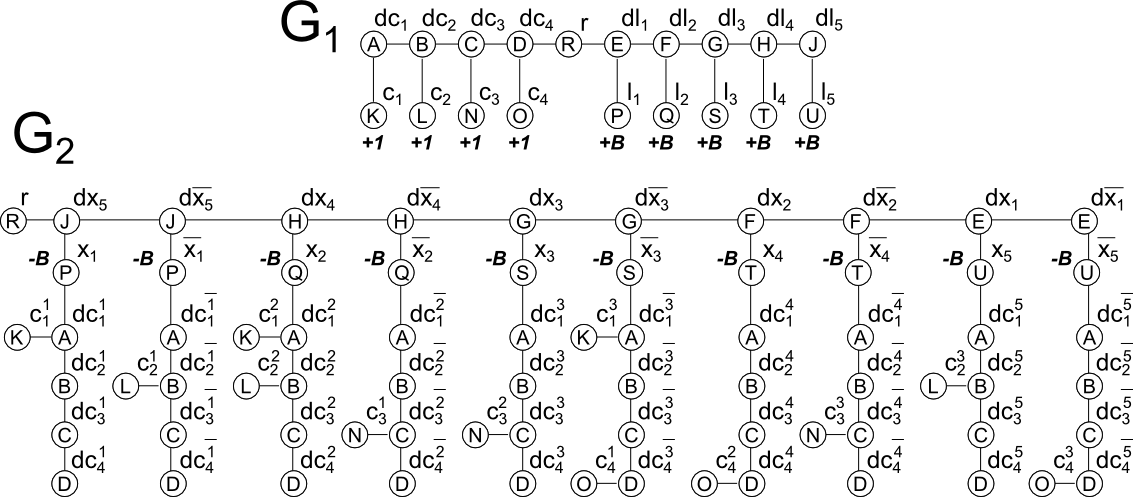
\includegraphics[width=\textwidth]{apx_bt-cater}
    	 	 \caption{Illustration of the construction of $G_1$, $G_2$, and $M$, given $C_q = \{(x_1 \vee x_2 \vee \neg{}x_3), (\neg{}x_1 \vee x_2 \vee x_5), (\neg{}x_2 \vee x_3 \vee \neg{}x_4), (\neg{}x_3 \vee x_4 \vee \neg{}x_5)\}$. For readability, the mapping $M$ is not drawn but represented as labels located on the nodes: any pair of nodes (one in $G_1$ and one in $G_2$) of similar inner label are mapped in $M$.}
			\label{fig:bt-cater}
		\end{figure}

		Let us prove that this construction is indeed an L-reduction from \msat{}. More precisely, we will prove the following property.
		\begin{lemma}
		There exists an assignment of $V_n$ satisfying at least $m$ clauses of $C_q$ if and only if there exists a solution to \mwccs{} of weight at least $m$.
		\end{lemma}

		\begin{proof}
		{\parindent0pt
		$\boxed{\Rightarrow}$ Given} an assignment $\mathcal{A}$ of $V_n$ satisfying $m$ clauses of $C_q$, we construct a solution to \mwccs{} of weight $m$ as follows.

		\begin{align*}
		\text{Let }V_1^*= &V_1 \setminus \{c_j ~\vert~ c_j\ \text{is not satisfied by the assignment}\}\text{ and}\\
		V_2^*= & \{r\} ~\cup \\
		& \{c^k_j ~\vert~ c_j \text{is satisfied by its } k\text{-th literal}\}  ~ \cup \\
		& \{x_i, dc^i_j ~\vert~ x_i=1, 1 \leq j \leq q\} ~\cup \\
		& \{\overline{x_i}, dc^{\overline{i}}_j ~\vert~ x_i=0, 1 \leq j \leq q\} ~\cup \\
		& \{dx_i,d\overline{x_i} ~\vert~ 1 \leq i \leq n\}.
		\end{align*}

		By construction, $G_1[V_1^*]$ is connected since all the vertices of the spine of the caterpillar have been kept. Moreover, $G_1[V_1^*]$ contributes $B \times n+m$ to the overall weight of the solution, that is $B$ for each of the $l_i$ and $+1$ for each satisfied clause.
		By construction, all the sub-trees rooted at $x_i$ (resp. $\overline{x_i}$) are kept in $G_2[V_2^*]$ if $x_i=1$ (resp. $x_i=0$) in $\mathcal{A}$. Moreover, all the dummy nodes for literals ($dx_i$ and $d\overline{x_i}$) and the root $r$ have been kept. Thus, $G_2[V_2^*]$ is also connected.
		Furthermore, $G_2[V_2^*]$ contributes to $-B\times n$ to the overall weight of the solution since exactly one of each variable node ($x_i$ and $\overline{x_i}$) has been kept. 
		One can easily check that any node of $V_1^*$ has a mapping counterpart in $V_2^*$. The overall solution is valid and of total weight $m$.

		\vspace*{1em}
		{\parindent0pt
		$\boxed{\Leftarrow}$ Given any solution $\{V_1^*,V_2^*\}$ to \mwccs{} of weight $m$, we construct a solution to the \msat{} problem satisfying at least $m$ clauses as follows.
		}

 	 	 First, note that we can assume that any such solution to \mwccs{} is \textit{canonical}, meaning that $V_2^*$ does not contain both vertices $x_i$ and $\overline{x_i}$ for all $1\leq i\leq n$. Indeed, by contradiction, suppose there exists a solution such that $\{x_i,\overline{x_i}\}\subseteq V_2^*$ for a given $1\leq i \leq n$. Then, $\{x_i,\overline{x_i}\}$ in $G_2$ induce a negative weight of $-2B$. This negative contribution can at most be compensated by the weight of the corresponding literal node in $G_1$ ($w_1(l_i)=B$) and at most $B$ clause nodes in $G_1$ ($B \geq \sum w_1(c_j)$ where $x_i\in c_j\ or\ \overline{x_i}\in c_j$) since every literal occurs in at most $B$ clauses in $C_q$. Therefore, such local configuration does not provide any positive contribution to the solution and can be transformed into a better solution by removing one of the sub-trees rooted in $\{x_i,\overline{x_i}\}$. We will consider hereafter that $m$ is the weight of the resulting canonical solution. We further assume that $m>1$ since otherwise we can build a trivial assignment $\mathcal{A}=\{c^1_1=1\}$ of $V_n$ that is satisfying at least one clause of $C_q$.

		Let $\mathcal{A}$ be an assignment of $V_n$ such that for all $1\leq i\leq n$ if $x_i\in V_2^*$ then $x_i=1$ and $x_i=0$ otherwise. Note that, since our solution is canonical, each literal has been assigned a single boolean value in $\mathcal{A}$. Let us now prove that this assignment satisfies at least $m$ clauses of $C_q$.

		First, note that since our solution is canonical and we require any node of $V_1^*$ to have a mapping counterpart in $V_2^*$, this implies that if $l_i\in V_1^*$ then its contribution (that is $w_1(l_i)=B$) is cancelled by the negative contribution of either $x_i$ or $\overline{x_i}$ in $V_2^*$ (that is $w_2(x_i)=w_2(\overline{x_i})=-B$). Therefore, the weight $m$ of the solution can only be realized by $m$ clause nodes of $G_1$, say $\mathcal{C}_1\subseteq V_1^*$ -- since $w_1(c_j)=1$ for all $1\leq j \leq q$.

		As already stated, to be part of the solution any node in $V_1^*$ has a mapping counterpart in $V_2^*$. Thus, for each node in $\mathcal{C}_1$, there should be a node of $\mathcal{C}_2 \subseteq \{c_j^k ~\vert~ 1\leq j \leq q, 1\leq k\leq 3\}$ in $V_2^*$. More precisely, by construction, any node $c_j$ in $V_1$ has exactly three mapping counterparts in $V_2$ (that is $\{c_j^k ~\vert~ 1\leq k \leq 3\}$) and for each $c_j\in \mathcal{C}_1$ at least one of these mapping counterparts has to belong to $\mathcal{C}_2$.

		Finally, since both $G_1[V_1^*]$ and $G_2[V_2^*]$ have to be connected, each node in $\mathcal{C}_2$, say $c_j^k$, should be connected by a path to a node $x_i$ or $\overline{x_i}$, say $x_i$, for some $1\leq i \leq n$, in $G_2[V_2^*]$. By construction, this is the case if $x_i$ is the $k$-th literal of the clause $c_j$ for some $1\leq k \leq 3$. Thus, $\mathcal{A}$ is an assignment that satisfies any clause $c_j$ such that the clause node $c_j$ belongs to $V_1^*$. As already stated $|\mathcal{C}_1|=m$.
		\end{proof}

		The above reduction linearly preserves the approximation since the weights of optimal solutions of the problems correspond and there exists an assignment of $V_n$ satisfying at least $m$ clauses of $C_q$ if and only if there exists a solution to \mwccs{} of weight at least $m$. Hence, given an approximation to \mwccs{}, one can derive an algorithm for \msat{} with the same approximation ratio. Since \msat{}, $B\geq 3$, is APX-hard \cite{papadimitriou1991optimization} and \msat{} for $B=6$ is not approximable within factor $1.0014$ \cite{berman1999some}, so is \mwccs{}, which proves Proposition \ref{sec:apx-bt-cater-proof}.

		Let us now prove a similar result for \mwccs{} problem when the mapping is a bijective function. 


		\subsection{Bijective relationship function, binary tree, and graph}
		\label{subsec:apx-bt-graph}

		XXX TODO: \emph{binary} tree, right now it's only with a general tree, need to include lots of dummies XXX


		\begin{proposition}\label{sec:apx-g-tree-proof}
  	  	  The \mwccs{} problem for a graph and a tree is APX-hard and not approximable within factor $1.0014$ even when the mapping is a bijective function and a complete conservation (i.e. $\alpha = 1$) is required.
		\end{proposition}

		Given any instance $(C_q,V_n)$ of \msat{}, we build a graph $G_1=(V_1,E_1)$ with weight function $w_1$, a tree $G_2=(V_2,E_2)$ with weight function $w_2$ and a mapping $M$ as follows. The graph $G_1$ has the vertex set $V_1=\{r, l_i, x_i, \overline{x_i}, c_j,$ $ c^k_j ~\vert~ 1\leq i\leq n, 1\leq j \leq q, 1\leq k \leq 3\}$ and the edge set defined by the following equation.
		\begin{align*}
		E_1= & \{(l_i,x_i), (l_i,\overline{x_i}), (r,x_i), (r,\overline{x_i}) ~\vert~ 1\leq i\leq n\} ~\cup  \\
 	 	 & \{(c_j,c_j^k), (r,c_j^k)  ~\vert~ 1\leq k \leq 3, 1\leq j \leq q\}.
		\end{align*}

		The weight function $w_1$ is defined as follows: for all $1\leq k \leq 3$, $1\leq i\leq n$ and $1\leq j \leq q$, $w_1(l_i)=B$, $w_1(c_j)=1$ and $w_1(r)=w_1(c_j^k)=w_1(x_i)=w_1(\overline{x_i})=0$.

		Roughly, in $G_1$ there is a node for each clause (denoted by $c_j$), for each of the three literals of each clause (denoted by $c_j^k$), for each literal (denoted by $l_i$) and for each valuation of each literal (denoted by $x_i$, $\overline{x_i}$). Clause nodes and literal nodes are separated by a central node $r$.

		The tree $G_2$ is defined as follows. The vertex set is $V_2=V_1$, the edge set is given by the following equation:
		\begin{align*}
		E_2= & \{(l_i,r), (c_j,r), (x_i,r), (\overline{x_i},r) ~\vert~ 1\leq i\leq n, 1\leq j \leq q\} ~\cup \\
		& \{(c^k_j,x_i) ~\vert~ x_i \text{ is the  } k\text{-th literal of clause } c_j\} ~\cup\\
		& \{(c^k_j,\overline{x_i}) ~\vert~ \overline{x_i} \text{ is the } k\text{-th literal of clause } c_j\}.
		\end{align*}

		The weight function $w_2$ is defined as follows: for all $1\leq k \leq 3$, $1\leq i\leq n$ and $1\leq j \leq q$, $w_2(x_i)=w_2(\overline{x_i})=-B$, $w_2(r)=w_2(c_j^k)=w_2(l_i)=w_2(c_j)=0$.


		Roughly, in $G_2$ all the nodes except the ones in $\{c_j^k~\vert~ 1\leq j \leq q, 1\leq k\leq 3\}$ form a star centered in node $r$. The nodes representing the literal of the clause (that is $c_j^k$) are connected to their corresponding variable nodes (that is $x_i$ or $\overline{x_i}$).

		Finally, the mapping $M$ is a bijective function from $V_1$ to $V_2$ defined as the identity (that is each node in $V_1$ is mapped to the node of similar label in $V_2$).


		\begin{figure}[ht]
    	 	 
    	 	 \centering
    	 	 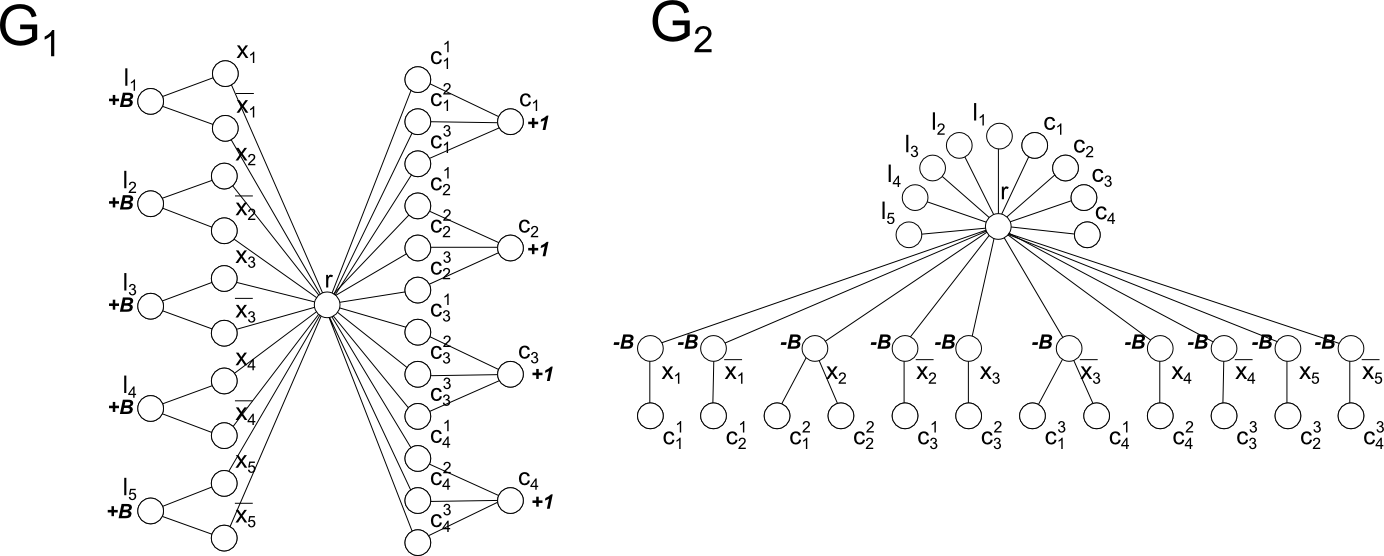
\includegraphics[width=\textwidth]{apx_g-tree}
    	 	 \caption{Illustration of the construction of $G_1$, $G_2$, and $M$, given $C_q = \{(x_1 \vee x_2 \vee \neg{}x_3), (\neg{}x_1 \vee x_2 \vee x_5), (\neg{}x_2 \vee x_3 \vee \neg{}x_4), (\neg{}x_3 \vee x_4 \vee \neg{}x_5)\}$. For readability, the mapping $M$ is not drawn but deduced from the labels of the nodes; any pair of nodes (one in $G_1$ and one in $G_2$) of similar label are mapped in $M$.}\label{fig:g-tree}
    	 	 \end{figure}
   		
		Let us prove that this construction is indeed an L-reduction from \msat{}. More precisely, we will prove the following property.

		\begin{lemma}
 	 	 There exists an assignment of $V_n$ satisfying at least $m$ clauses of $C_q$ if and only if there exists a solution (not necessarily optimal) to \mwccs{} of weight at least $m$.
		\end{lemma}

		\begin{proof}

		{\parindent0pt
		$\boxed\Rightarrow$} Given an assignment $\mathcal{A}$ of $V_n$ satisfying $m$ clauses of $C_q$, we construct a solution to \mwccs{} of weight $m$ as follows.

		Let $V_1^*=V_2^*=\{c_j~\vert~ c_j \text{ is satisfied by } \mathcal{A}\} \cup \{c^k_j~\vert~ c^k_j \text{ is satisfying } c_j \text{ by } \mathcal{A}\}\cup\{x_i~\vert~ x_i=1\}\cup\{\overline{x_i}~\vert~ x_i=0\}\cup \{r,l_i~\vert~ 1\leq i\leq n\}$. 

		By construction, $G_1[V_1^*]$ and $G_2[V_2^*]$ are connected. Moreover, $G_1[V_1^*]$ contributes $B\times n+m$ to the overall weight of the solution, that is $B$ for each of the $l_i$ and $+1$ for each satisfied clause, while $G_2[V_2^*]$ contributes $-B\times n$ to the overall weight of the solution since exactly one of each variable node ($i.e.$, $x_i$ and $\overline{x_i}$) has been kept. The overall solution is valid and of total weight $m$.

		\vspace*{1em}
		{\parindent0pt
		$\boxed{\Leftarrow}$} Given any solution $V^*\subseteq V_1$ to \mwccs{} of weight $m$, we construct a solution to the \msat{} problem satisfying at least $m$ clauses as follows.

		First, note that, as in the previous construction, we can assume that any such solution to \mwccs{} is \textit{canonical} meaning that $V^*$ does not contain both vertices $x_i$ and $\overline{x_i}$ for any $1\leq i\leq n$.

		Let $\mathcal{A}$ be an assignment of $V_n$ such that for all $1\leq i\leq n$, if $x_i\in V^*$ then $x_i=1$ and $x_i=0$ otherwise. Note that, since our solution is canonical, each literal has been assigned a single boolean value in $\mathcal{A}$. Let us now prove that this assignment satisfies at least $m$ clauses of $C_q$.

		First, note that since our solution is canonical, as in the previous construction, the weight $m$ of the solution can only be induced by $m$ clause nodes of $G_1$, say $\mathcal{C}_1\subseteq V^*$.

		Since both $G_1[V^*]$ and $G_2[V^*]$ have to be connected, any solution with $m>1$ will include node $r$ in $V^*$. Thus, for each node $c_j\in\mathcal{C}_1$ there should be a node of $\{c_j^k ~\vert~ 1\leq k\leq 3\}$ in $G_1[V^*]$ to connect $c_j$ to $r$. In $G_2[V^*]$, in order for nodes $r$ and $c_j^k$ to be connected, the corresponding literal node (that is $x_i$ or $\overline{x_i}$), say $x_i$ -- has to be kept in $V^*$. By construction, this is the case if $x_i$ is the $k$-th literal of clause $c_j$. Thus, $\mathcal{A}$ is an assignment that satisfies any clause $c_j$ such that the clause node $c_j$ belongs to $V^*$. As already stated $|\mathcal{C}_1|=m$.
		\end{proof}

		The above reduction linearly preserves the approximation and proves Proposition \ref{sec:apx-g-tree-proof}.

	\section{Polynomial-time cases for the \mwccs{} problem}
	\label{sec:poly}


		\subsection{Two trees and a bijective mapping}
		\label{subsec:tree1o1}

			Here we continue to explore the case with fixed $\alpha = 1$.
			We have proved in \cref{subsec:apx-bt-cater} that on instances with two binary trees, and an injective mapping function, the problem is APX-hard.
			We will now consider the case of two general trees, $T_1 = (V_1, E_1)$ and $T_2 = (V_2, E_2)$, with a bijective relationship $V_1\,M\,V_2$.

			The standard algorithms for \mwcs{} and its variants\footnote{Mainly cardinality-constrained, budget-constrained, and ratio-bounded, with a pseudo-polynomial algorithm for all of them exposed in the next chapter.} use bottom-up, usually dynamic-programming, approaches.
			Given an unrooted tree $T$, root $T$ in one of its node to direct the edges.
			Then, compute recursively the maximum weight of the subtrees that unconditionally includes their root.

			It would be a good characteristic of our algorithm to advance in a similar fashion, recursively solving subproblems, and progressing in both trees in locked step.
			However in our case, the mapping function defines a strong constraint on the possible steps since $\alpha=1$, and a node can only be selected if its counterpart is.
			Furthermore, a node in one tree can have its counterpart at a completely different level in the other, leading to some difficulty in finding a viable locked-step advancement scheme.
			This last point make impossible to devise a local recursive procedure to find the optimal subtree.
			Indeed, adding a child node might require the addition of a parent by mutual requirement between the two trees and the mapping function, see \cref{fig:childReqParent} for an exemple.

			\begin{figure}[ht]
				\centering
				%\includegraphics[width=\textwidth]{}
				\label{fig:childReqParent}
				\caption{XXX image with mapping from root to leaf in both trees: locked-step require to take two full paths at the same time XXX}
			\end{figure}

			We will use the fact that we require a perfect matching to drive the steps from one of the two trees, say $T_1$.
			Indeed, selecting a node in $T_1$ requires the unconditional inclusion of its counterpart in $T_2$, and of all node required to connect them, this until no more nodes require to be included.

			This last operation, $\text{ConstructRequiredSet}$, is defined as follows.
			Given two non-empty sets $S_1$ and $S_2$ of nodes already selected in $V_1$ and $V_2$, and a node $u \in V_1 \setminus S_1$ such that $u$ is a neighbor of a node in $S_1$, $v \in V_2$ its counterpart.
			We will define a double recursion procedure that will work first with $V_1$, then with $V_2$.
			Add $u$ to $S_1$; then, find the shortest path from $v$ to any node of $S_2$.
			Add all nodes that pertain to this shortest path to $S_2$, and recursively find all shortest paths from the counterparts of those nodes to the nodes of $S_1$.
			Continue until no more nodes need to be added.

			\begin{proposition}\label{sec:apx-bt-cater-proof}
				The induced graphs $T_1[S_1]$ and $T_2[S_2]$ obtained as results of $\text{ConstructRequiredSet}$ are connected.
			\end{proposition}
			\begin{proof}
				Indeed, since we recursively add nodes with their shortest path to already selected nodes, their exists a path connecting every pairs of nodes of $S_1$ and of $S_2$.
			\end{proof}

			\begin{proposition}\label{sec:apx-ater-proof}
				$\text{ConstructRequiredSet}$ is a quadratic operation in the worst case.
			\end{proposition}
			\begin{proof}
				The shortest path in a tree is equivalent to the minimum sum subsequence problem XXX ref XXX and can be solved in linear time.
				We recursively add up the nodes up to $2n$.
				Hence the resulting complexity.
			\end{proof}

			The main procedure is a recursive decision tree traversal that will be using the $\text{ConstructRequiredSet}$ operation.
			This recursive procedure, $\text{ComputeDecisionTree}$ is defined as follows.
			Given two sets $S_1$ and $S_2$ of connected nodes in $V_1$ and $V_2$ respectively.
			Define $C$ as the union of all children of the nodes in $S_1$.
			For all nodes $c \in C$, call the $\text{ConstructRequiredSet}$ procedure with $S_1$, $S_2$ and $c$, which will return $S',1$ and $S'_2$.
			Continue the construction of the decision tree by recursively calling $\text{ComputeDecisionTree}$ with $S'_1$ and $S'_2$ until there are no more children.
			Note that the score of a node in the decision tree is equal to the sum of the scores of its children minus the score of the nodes that are in common.

			\begin{figure}[ht]
				\centering
				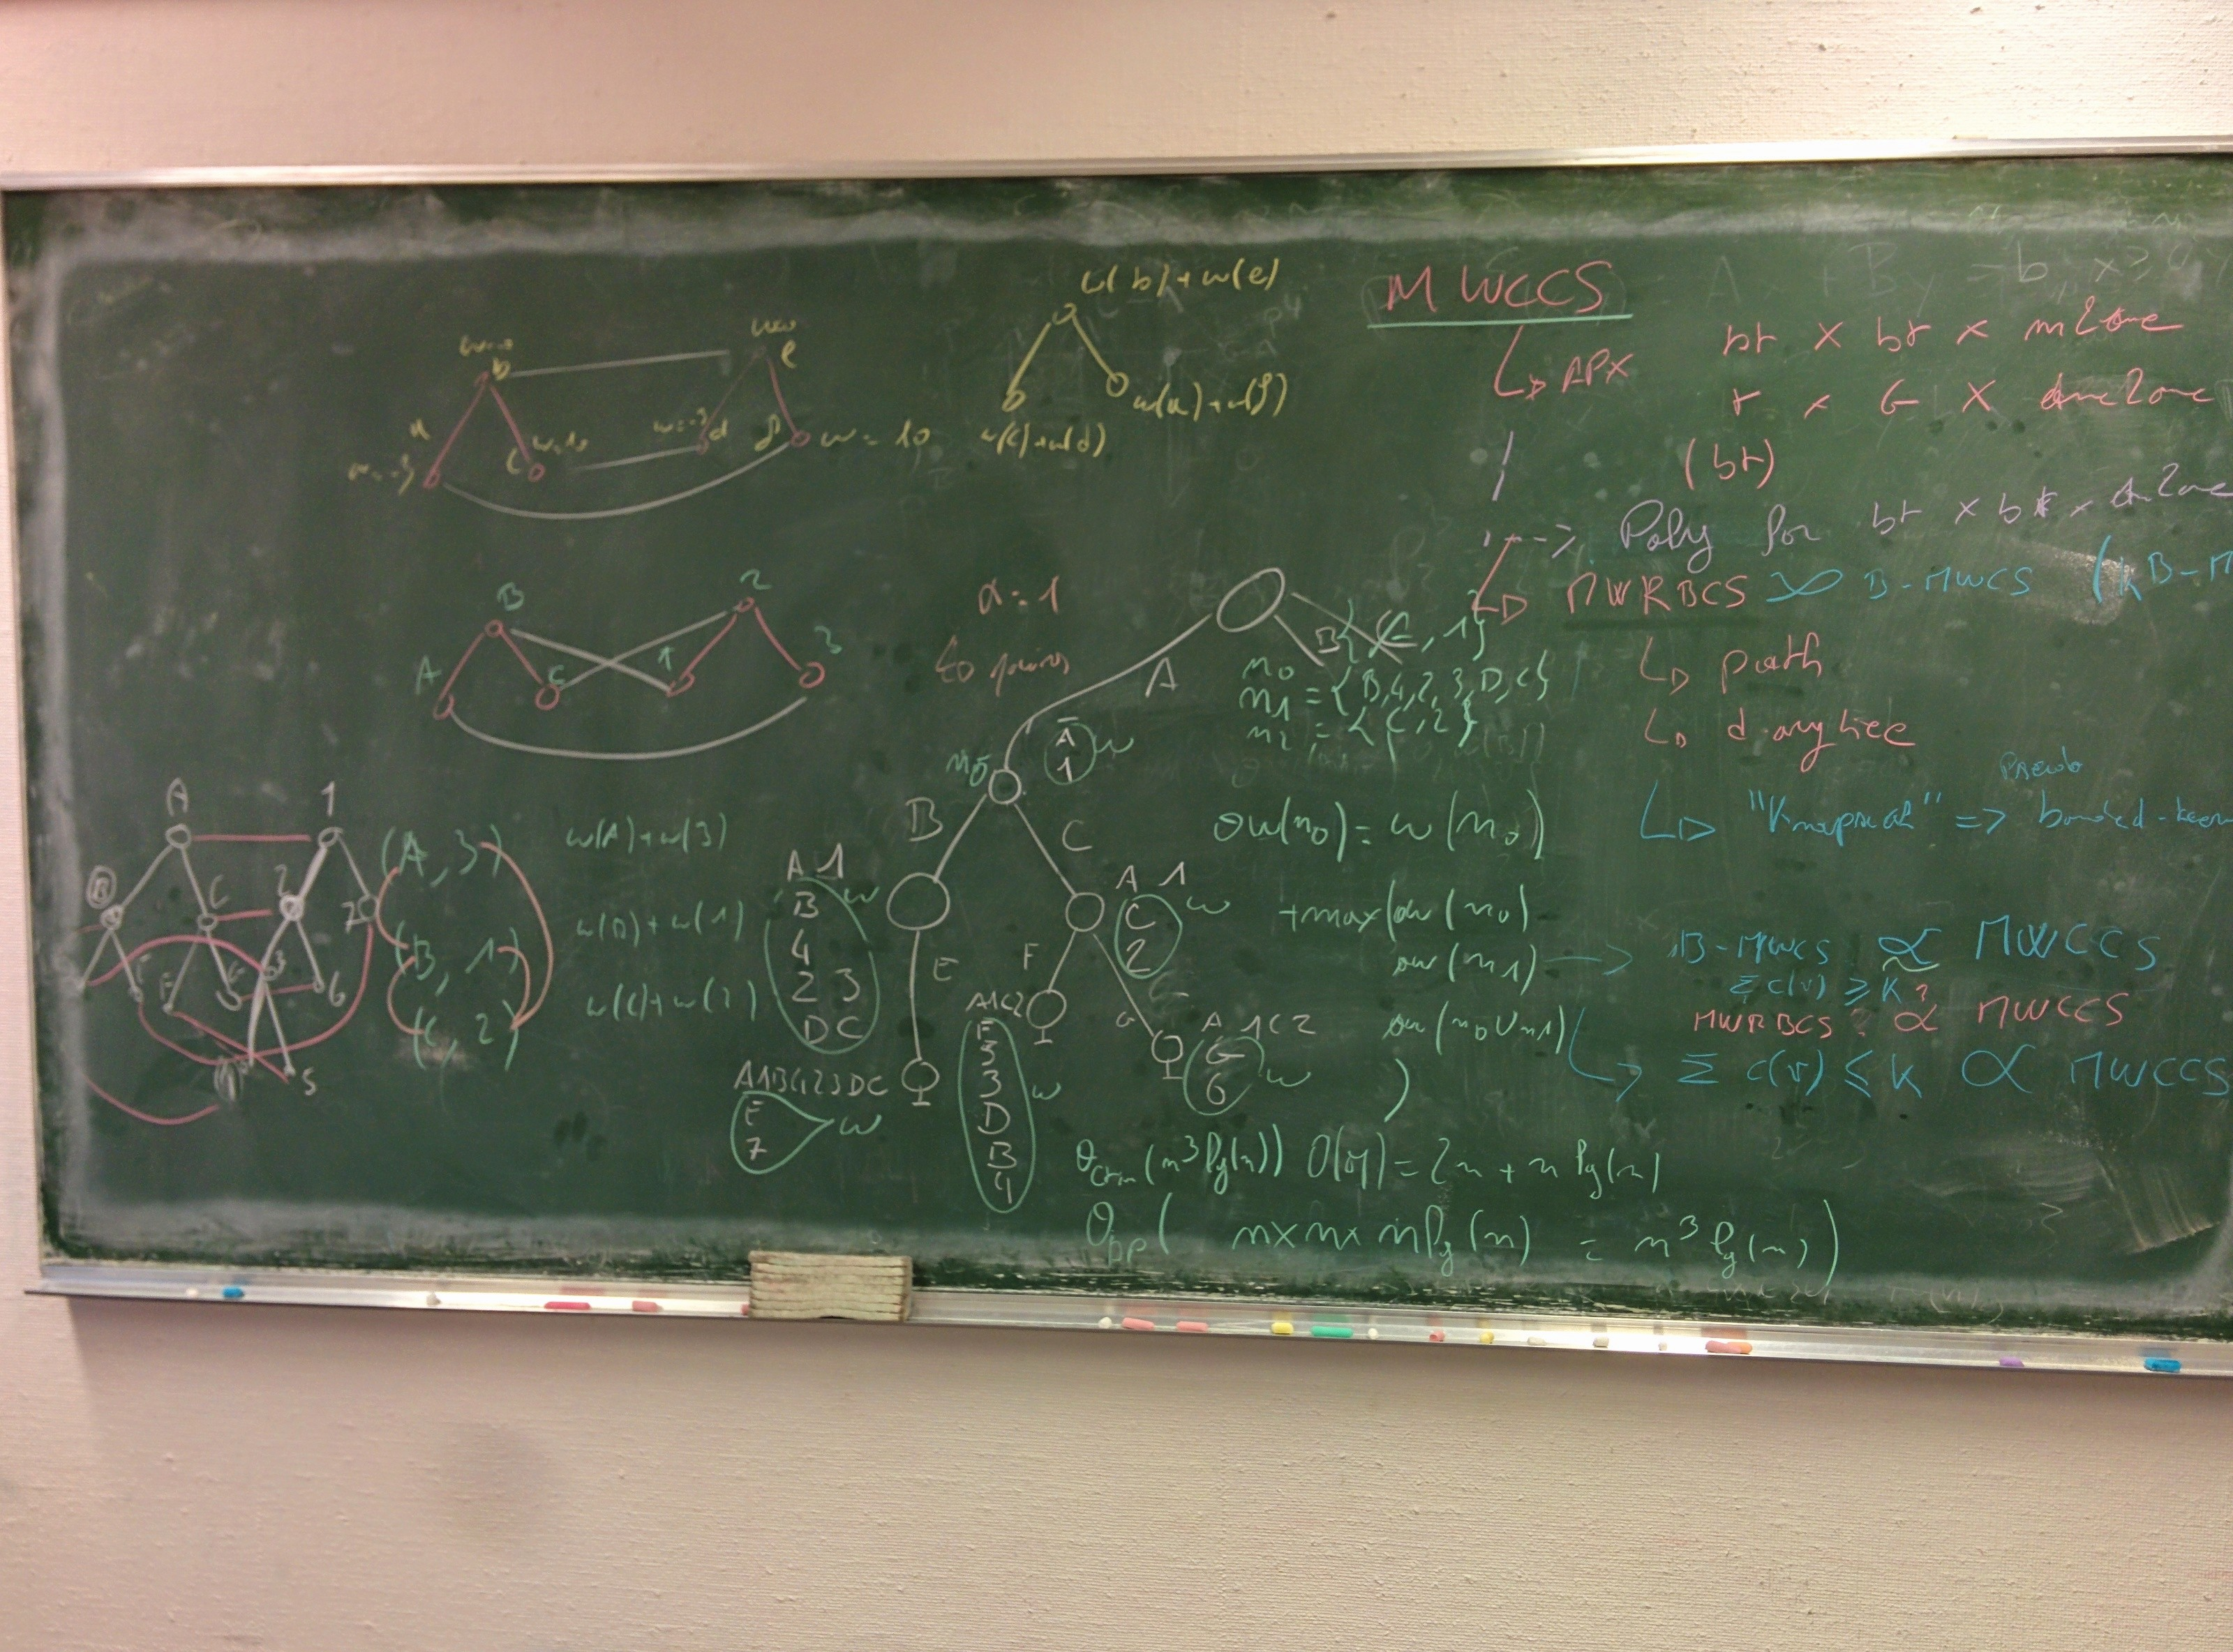
\includegraphics[width=\textwidth]{IMG_20141216_163836}
				\label{fig:foo}
			\end{figure}

			XXX Drawing version of the example on the board XXX

			\begin{proposition}\label{sec:apx-bt}
				$\text{ComputeDecisionTree}$ requires at most $O(n^3\lg(n))$ steps.
			\end{proposition}
			\begin{proof}
				The decision tree contains $\prod_{i=n-1}^{1}{n} = O(n^2)$ nodes in the worst case.
				To compute the score, it is required to compute the set union operation, which is an $O(n\lg(n))$ operation with tree representation of the sets.
				Hence the resulting number of steps.
			\end{proof}

			Finally, note that this procedure can lead to different results depending on the starting set $S_1$ and $S_2$.
			The final step is to construct the decision tree for all pairs $u,v \in V_1\times V_2$, and select the optimal solution.

			\begin{proposition}\label{sec:at-cater-proof}
				This last procedure is linear in the number of nodes.
			\end{proposition}
			\begin{proof}
				Indeed, since the nodes are on a one to one mapping, there exists exactly $\norm{V_1} = \norm{V_2}$ such pairs.
			\end{proof}


			XXX Need to find an example and make a figure XXX
			

		\subsection{Polynomial-time scheme for some inputs}
		\label{subsec:enumerable}

			Here we consider the general version of the \mwccs{} problem where $\alpha$ is given as input rather than being fixed.
			In addition, we further relax the constraint on the relationship function, which can be any partial injective function.
			That is, any element of $V_1$ can have at most one image in $V_2$ (the elements of $V_2$ can have 0, 1, or more antecedents).
			Finally, we suppose that there is a polynomial number of connected induced subgraphs of $G_1$.

			We will consider as many candidate solution as there are connected subgraphs of $G_1$, and for each one of them we will try to find the best corresponding subgraph in $G_2$.
			The best corresponding subgraph in $G_2$ is the subgraph that maximizes the total weight of the candidate solution and such that at least an $\alpha$-fraction of the nodes of $G_1$ and $G_2$ in the solution are $M$-related.
			For a given subgraph of $G_1$, the sum of its nodes' weight is fixed, hence maximizing the total weight of the candidate solution is equivalent to finding the optimal solution in $G_2$ where the $\alpha$-fraction constraint holds.

			To solve this problem, we introduce a new problem, the \textsc{ratio-bounded maximum-weight connected subgraph} (\rbmwcs) problem, for which the formal definition and detailed analysis are provided in the next chapter.
			Informally, it consists in a variant of the \mwcs{} problem where an additional contribution function is associated to each node and where an additional ratio constraint is introduced\footnote{not unlike the \emph{budget-constrained} variant of the \mwcs{} problem, cf. next chapter for more details}.

			The reduction to this new subproblem is as follows.
			The contribution function needs to \emph{encode} the relationship function between the nodes of both $G_1$ and $G_2$.
			To do so, and since we fixed a partial solution to the problem in the form of the subgraph of $G_1$, we note for each node of $G_2$ its number of inverse images in $G'_1$ plus one if and only if at least one exists, zero otherwise.
			The reason we need to make the distinction between the two cases is that when there is no counterpart in $G_1$, selecting a node in the optimal solution in $G_2$ will not increase the number of mapped node overall.
			However, selecting a node in $G_2$ for which there exists at least one counterpart will increase the number of mapped node by the number of counterpart, plus one for the selected node itself.

			Formally, given a connected subgraph $G'_1=(V'_1,E'_1)$ of $G_1$, we define the corresponding $G_2$ \emph{antecedent function} $a\colon V_2 \to \mN$ to be $a(v)=\card{\Set{v,u}{M(u,v), u\in V'_1}}$.
			The \emph{contribution function} $c\colon V_2 \to \mN$ is defined as follows:
			$$c(v)=\begin{cases}a(v) + 1 &\mbox{if }a(v) > 0\mbox{,} \\
		                       0        &\mbox{otherwise.}
		          \end{cases}$$

			Given $G_2=(V_2,E_2)$, its weight-function $w_2$ and its contribution function $c$, the problem now corresponds to the discovery of the connected subgraph of maximum weight such that:
			\begin{align*}
				\sum_{v \in V^*_2}{c(v)}                           &\geq \alpha\times\left(\norm{V'_1} + \norm{V^*_2}\right) \\
				\sum_{v \in V^*_2}{c(v)} - \alpha\times\norm{V'_1} &\geq \alpha\times\norm{V^*_2}
			\end{align*}
			Where $\alpha\times\norm{V_1'}$ is constant.

			Finally, given the optimal score of all candidate solutions, for which there are one for each subgraphs $G'_1$, the optimal solution to the \mwccs{} problem is the one candidate solution among them which has the best score.

			Clearly, constructing a contribution function for $G_2$ given a subgraph $G'_1$ is a linear time operation. Choosing the best candidate solution is as time consuming as enumerating all subgraphs of $G_1$, which is a polynomial time operation in this context. The complexity of this algorithm hence depends on the difficulty to solve the \rbmwcs{} subproblem.

			\Cref{chap:rbmwcs} provides a detailed analysis of this problem with a more general contribution function.
			It provides pseudo-polynomial scheme for all classes of input graphs up to bounded treewidth.
			However, when the contribution function is enumerable with a polynomial upper bound, and such is the case by construction here, the scheme actually becomes a polynomial-time algorithm.
			Thus, there exists a polynomial-time algorithm to solve \mwccs{} when one of the graph if polynomially enumerable, the second is bounded treewidth, and the relationship is a partial injective function, for any $\alpha \in [0, 1]$.
